

%ei varmaan saa olla kysymy
\subsubsection{Mikä on React}

%ei saa olla metatekstiä
%https://github.com/facebook/react/blob/main/README.md
%https://www.infoq.com/news/2013/06/facebook-react/
% molemmat siteerattu 27.5.24


% ei ole metan kehittämä vaan se on vaan ylläpitämä. facebookin työntekijä teki sen
React on metan kehittämä ja ylläpitämä avoimeen lähdekoodiin perustuva javascript kirjasto, joka on suunniteltu reaktiivisien käyttöliittyjien kehittämiseen.
%more text

%rnative selitys paremmin
reaktia voi käyttää web ja mobiili käyttöliittymien tekemiseen react nativella
%vitusti lisää tekstiä
\medskip








\subsubsection{jsx}

%https://react.dev/learn/writing-markup-with-jsx
%https://facebook.github.io/jsx/ 

% jsx = js xml
% https://medium.com/@sjarancio/what-is-jsx-e3dda0af3490

%transpilation
%https://www.scholarhat.com/tutorial/react/getting-started-with-jsx
% https://www.typescriptlang.org/docs/handbook/jsx.html

% kaikki viitattu 27.5

%html koodia uusiks
JSX (javascript XML) on sytaksi jatke javascriptille, joka antaa kehittäjän kirjoittaa html tyylistä koodia javascriptin sekaan
% asiakielellä
selain ei itse osaa lukea jsx koodia joten se pitää transpiloida javascriptiksi ennen kun sen voi deploy



% suora sitaatti https://facebook.github.io/jsx/ 
JSX ei ole ECMAscript standardissa, joten selaimet eivät osaa tulkita sitä, vaan JSX se on suunniteltu transpiloitavaksi johonkin ECMAscript standardia toteuttavalle kielelle
\medskip

\bigskip
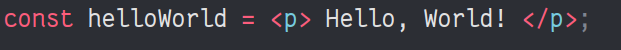
\includegraphics[width=10cm]{src/public/oppar/pure_jsx_example.png}

Kuva\getImgCount .{} kuvankaappaus JSX syntaxista.
\medskip

Kuvassa luodaan elementti helloWorld, jolle annetaan arvoksi paragraafi, jossa teksti "Hello, World!"{}.
% loppu pitää kirjottaa jotenkin paremmin ja pitää yhistää paremmin 
Elementtien arvot voidaan kirjoittaa html tyylillä, joka tekee jutuista kivaa.
\medskip



\bigskip
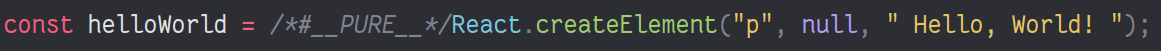
\includegraphics[width=15cm]{src/public/oppar/transpiled_jsx_example.png}

Kuva\getImgCount .{} Kuvankaappaus helloWorld elementistä, joka on käännetty javascriptiin. 
\medskip

%vähän toistoa muttei väliä sillä pitää siteerata tämä

%https://babeljs.io/repl 
kuvassa on helloworld elementti, joka on käännetty natiiviksi javascriptiksi babel kääntäjää käyttäen.
Tämä antaa selaimille mahdollisuuden tulkita JSX koodia.
%jotain lisää
\medskip

% https://github.com/facebook/react/blob/a4195750779dbd9a13e1615fbbd493bf2c5768ca/packages/react/src/ReactElement.js#L362
%pitää vissii kysyy voiko lähdekoodia käyttää lähteenä..


\subsubsection{Komponentit}


%https://react.dev/learn/your-first-component

Oma tekemä komponentti. se voi sisältää tilaa ja kutsuja muihin komponentteihin jne
komponentteihin voi lisätä interaktiivisuutta jne



komponentit on vähän niinkuin oma elementti jonkqa voi kirjoittaa jsx koodiin siististi

\medskip

\subsubsection{Reaktin struktuuri ja toiminta}


index.js lähtien

%https://react.dev/reference/react-dom/client/createRoot
% viittaus 29.5

%laitetaanko kuva jostain indexistä
%vaikka joku joka on tehty create react app jutulla


reactdom createroot
react tekee funktiolle antamasta elementistä Root elementin, ja se alkaa hallinnoimaan domia sen alla
\medskip

%jos nämä yhdistää tarvitaan toinen kappale. voitaisiin tosin kirjoittaa muutenkin toinen kappale toiminnasta. tai koko lifecyclestä
% ainakin jos mainitaan vdomista joitan

root.render
render funktio suorittaa komponentin funktiona. komponentti on jo tässä vaiheessa käännettu natiiviksi javascriptiksi, 
joten komponentin lapsikomponentit voidaan suorittaa samalla. Lopputuloksena saadaan natiivi html elementtejä jotka selain voi renderöidä.

\medskip



%joku maininta vdomista jossain vaiheessqa enne ntätä ja sitten siirrä oikeaan paikkaan
\subsubsection{DOM ja VDOM}


%jotain domista, mikä se on ja miten se liittyy käyttöliittymiin ja sitten mikä on vdom
% vai pitäisikö samantien aloittaa että meillä on vdom, ja sittem selittää mikä dom on..... kuulostaa väärältä

% https://www.w3.org/TR/WD-DOM/introduction.html
% 29.5


%psychotic
DOM (eng Document object model) on puu-struktuurinen representaatio HTML dokumentista.
Tätä struktuuria käytetään rajapintana JavaScriptin ja HTML:län välillä. 
Struktuurissa jokainen solmu on objekti, joka esittää osaa dokumentista. 
Soulmuissa voi olla yksi tai useampi objekti ja nämä objektit voivat osoittaa muihin solmuihin.



esimerkiksi dom representaatio seuraavasta html koodista

% https://www.w3.org/TR/WD-DOM/introduction.html
% kuva ja koodi molemmat täältä.. 29.5 viitatti
    
%pitää viitata jotenkin
\begin{tcolorbox}
\begin{lstlisting}[language=html]
<TABLE>
    <ROWS> 
      <TR> 
          <TD>Shady Grove</TD>
          <TD>Aeolian</TD> 
      </TR> 
      <TR>
          <TD>Over the River, Charlie</TD>
          <TD>Dorian</TD> 
      </TR> 
    </ROWS>
</TABLE>
\end{lstlisting}
\end{tcolorbox}


Esimerkki HTML koodissa luomme pöydän, jossa tehdään kaksi riviä ROWS elementin alle. 
%sisältää väärä sana
Joka riviin tulee kaksi "table data"{} elementtiä, jotka sisältää datan tekstinä.
\bigskip



%kuva html domista
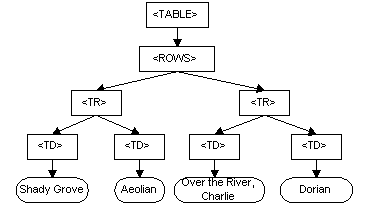
\includegraphics{./src/public/oppar/dom.png}

Kuva\getImgCount .{} DOM puu esimerkki HTML koodista. Jonathan Robie, Texcel Research 
\medskip

Kuvassa on esimerkki HTML koodista tehty DOM puu struktuuri.
tätä käyttämällä, 

jotain rajapinta interaktiivisuus helppokäyttöisyys javascript jne lorem ipsum lorem ipsumlorem ipsumlorem ipsumlorem ipsum

\bigskip



%https://medium.com/@BharathkumarV/reacts-virtual-dom-17fdcb290a10
% siteerattu 27.5

VDOM (eng Virtual Dom) on virtuaalinen esitys DOM:ista, jonka react pitää musitissaan koko suorituksen ajan.
VDOM:ia käyttäen react voi nopeasti päätellä mitkä osat käyttöliittymästä pitää päivittää, kun jonkun komponentin tila päivittyy. 
\medskip



